\documentclass[sigconf]{acmart}

\usepackage{listings}
\usepackage{booktabs}
\usepackage{graphicx}

% Copyright
%\setcopyright{none}
%\setcopyright{acmcopyright}
%\setcopyright{acmlicensed}
\setcopyright{rightsretained}
%\setcopyright{usgov}
%\setcopyright{usgovmixed}
%\setcopyright{cagov}
%\setcopyright{cagovmixed}

%% Comments
\newif\ifcomments\commentsfalse

\ifcomments
\newcommand{\authornt}[3]{\textcolor{#1}{[#3 ---#2]}}
\newcommand{\todo}[1]{\textcolor{red}{[TODO: #1]}}
\else
\newcommand{\authornt}[3]{}
\newcommand{\todo}[1]{}
\fi

\newcommand{\ds}[1]{\authornt{red}{DS}{#1}} %Dan
\newcommand{\wss}[1]{\authornt{blue}{SS}{#1}} %Spencer
\newcommand{\jc}[1]{\authornt{magenta}{JC}{#1}} %Jacques
\newcommand{\spr}[1]{\authornt{green}{SP}{#1}} %Steven
\newcommand{\jtol}{$J_{\mbox{tol}}$}
\newcommand{\inlHask}[1]{\lstinline[language=Haskell, columns=fullflexible,
  basicstyle=\ttfamily, showstringspaces=false, breaklines=true]{#1}}
% DOI
%\acmDOI{10.475/123_4}

% ISBN
%\acmISBN{123-4567-24-567/08/06}

%Conference
\acmConference[SE-CSE\_SE-CoDeSE]{2017 International Workshop on Software Engineering
  for High Performance Computing in Computational and Data-Enabled Science and
  Engineering}{November 2017}{Denver, Colorado, USA} 
\acmYear{2017}
\copyrightyear{2017}

%\acmPrice{15.00}

\begin{document}
\title[Drasil Framework]{Drasil: A Framework for Scientific Knowledge Capture and Artifact Generation}

\author{Daniel Szymczak}
\affiliation{%
  \institution{Computing and Software Department, McMaster University}
  \streetaddress{1280 Main Street West}
  \city{Hamilton} 
  \state{Ontario} 
  \postcode{L8S 4K1}
}
\email{szymczdm@mcmaster.ca}

\author{Spencer Smith}
\affiliation{%
  \institution{Computing and Software Department, McMaster University}
  \streetaddress{1280 Main Street West}
  \city{Hamilton} 
  \state{Ontario} 
  \postcode{L8S 4K1}
}
\email{smiths@mcmaster.ca}

\author{Jacques Carette}
\affiliation{%
  \institution{Computing and Software Department, McMaster University}
  \streetaddress{1280 Main Street West}
  \city{Hamilton} 
  \state{Ontario} 
  \postcode{L8S 4K1}
}
\email{carette@mcmaster.ca}

\author{Steven Palmer}
\affiliation{%
  \institution{Computing and Software Department, McMaster University}
  \streetaddress{1280 Main Street West}
  \city{Hamilton} 
  \state{Ontario} 
  \postcode{L8S 4K1}
}
\email{palmes4@mcmaster.ca}

\begin{abstract}
What if building \emph{well-documented} software was not tedious and unrewarding?  We
are implementing a framework, Drasil, to greatly alleviate these issues. Here
we document the design and development process of Drasil.  We show, through a case
study (GlassBR -- for computing the safety of glass panes with respect to
explosions), how Drasil can be used. While software like GlassBR is algorithmically
straightforward, it is used in safety related applications, which makes its correctness
quite important. For Drasil, the context we are most interested in is when correctness is
established within the context of \emph{software certification}.

Our principal means of producing documentation is through weaving together
standardized knowledge, as captured in Drasil.  We illustrate how this makes
scientific software development more transparent, and increases reusability and
reproducibility.
\end{abstract}

%
% The code below should be generated by the tool at
% http://dl.acm.org/ccs.cfm
%

\begin{CCSXML}
<ccs2012>
<concept>
<concept_id>10010405.10010497.10010510</concept_id>
<concept_desc>Applied computing~Document preparation</concept_desc>
<concept_significance>300</concept_significance>
</concept>
<concept>
<concept_id>10010405.10010432</concept_id>
<concept_desc>Applied computing~Physical sciences and engineering</concept_desc>
<concept_significance>100</concept_significance>
</concept>
<concept>
<concept_id>10011007.10011006.10011041.10011047</concept_id>
<concept_desc>Software and its engineering~Source code generation</concept_desc>
<concept_significance>300</concept_significance>
</concept>
<concept>
<concept_id>10011007.10011074.10011092</concept_id>
<concept_desc>Software and its engineering~Software development techniques</concept_desc>
<concept_significance>300</concept_significance>
</concept>
<concept>
<concept_id>10011007.10011074.10011092.10011096</concept_id>
<concept_desc>Software and its engineering~Reusability</concept_desc>
<concept_significance>300</concept_significance>
</concept>
<concept>
<concept_id>10011007.10011074.10011092.10011782</concept_id>
<concept_desc>Software and its engineering~Automatic programming</concept_desc>
<concept_significance>300</concept_significance>
</concept>
<concept>
<concept_id>10011007.10011074.10011099.10011105.10011110</concept_id>
<concept_desc>Software and its engineering~Traceability</concept_desc>
<concept_significance>300</concept_significance>
</concept>
<concept>
<concept_id>10002950.10003705</concept_id>
<concept_desc>Mathematics of computing~Mathematical software</concept_desc>
<concept_significance>100</concept_significance>
</concept>
<concept>
<concept_id>10003456.10003457.10003580.10003585</concept_id>
<concept_desc>Social and professional topics~Testing, certification and licensing</concept_desc>
<concept_significance>100</concept_significance>
</concept>
</ccs2012>
\end{CCSXML}

\ccsdesc[300]{Applied computing~Document preparation}
\ccsdesc[100]{Applied computing~Physical sciences and engineering}
\ccsdesc[300]{Software and its engineering~Source code generation}
\ccsdesc[300]{Software and its engineering~Software development techniques}
\ccsdesc[300]{Software and its engineering~Reusability}
\ccsdesc[300]{Software and its engineering~Automatic programming}
\ccsdesc[300]{Software and its engineering~Traceability}
%\ccsdesc[100]{Mathematics of computing~Mathematical software}
\ccsdesc[100]{Social and professional topics~Testing, certification and licensing}


\keywords{scientific computing, software quality, software engineering, document
driven design, code generation, software certification}

\maketitle

\section{Introduction} \label{SecIntroduction}

Every developer should strive for software of the highest possible quality,
especially for safety-related applications, where incorrect software could
cost lives. As scientists, we should be leading the community in developing high
quality software; our duty is to ensure the reusability, reproducibility, and
replicability of our work.

Our team is focused on improving the quality of Scientific Computing Software (SCS).
We have chosen large, multi-year, multi-developer projects where quality is
sufficiently important that \emph{certification} may be sought.  In this 
domain, the end users do much of the development. For these projects, we pay
particular attention to improving the qualities of reusability, reproducibility,
and certifiability. 

The goal for software certification is to: ``...systematically determine, based
on the principles of science, engineering and measurement theory, whether a
software product satisfies accepted, well-defined and measurable criteria''
\cite[p.~12]{HatcliffEtAl2009}.  We aim to streamline the certification process,
by simplifying the creation of the requisite software artifacts (documentation
and code) and by ensuring these artifacts are always consistent. Tracking
down the source of any information contained in our artifacts should be
trivially easy.  This is rarely the case (currently), as documentation is often
not a high priority.

Improved documentation is often considered too high a cost in terms of time and 
effort for SCS developers, particularly when dealing with rapid changes in 
requirements. However, it is an important aspect of improving overall software 
quality. Carver~\cite{CarverEtAl2007} observed that scientists do not view 
rigid process-heavy approaches favourably. Moreover, others have observed that
SCS developers tend to dislike producing documentation~\cite[p.~373]{Roache1998}.

Previous work by Smith \& Koothoor~\citep{SmithAndKoothoor2016} found $27$
errors in an existing safety-related software package (nuclear safety analysis
software) when re-documenting the software using a rigorous approach. Had they
attempted to certify the software, most, if not all, of these errors would have
led to a failure.

Well-maintained documentation provides numerous advantages including:
\begin{itemize}
\item Improved software qualities:
    \begin{itemize}
    \item Verifiability
    \item Reusability
    \item Reproducibility
    \end{itemize}

\item Other improvements (from Parnas~\cite{Parnas2010}):
    \begin{itemize}
        \item Easier reuse of old designs
        \item Better communication about requirements
        \item More useful design reviews
    \end{itemize}
\end{itemize}

Developers are being made aware of the advantages of 
documentation~\cite{SmithJegatheesanAndKelly2016}. Yet it can still be difficult 
to realize these advantages because documenting software is typically 
felt to be:

\begin{itemize}
\item Too time consuming,
\item Too difficult to maintain,
\item Not amenable to change,
\item Too tied to the waterfall process, and
\item Counterproductive when reporting on each stage of 
        development~\cite{Roache1998}.
\end{itemize}

There are also other issues with document-rich, certifiable software 
development. Namely the vast amount of knowledge duplication across software 
artifacts. Consider a simple piece of software with the following artifacts:

\begin{itemize}
\item Software Requirements Specification (SRS),
\item Design Document,
\item Source Code, and
\item Tests.
\end{itemize}

Knowledge such as the functional requirements from the SRS is duplicated in 
both the source code and tests. That same knowledge appears in the design 
document as well, albeit in a different form. 

Software certification typically requires many more 
artifacts than the four listed above. Much of the same knowledge, possibly in a
variety of representation, will appear in the artifacts and will need to be
maintained. Manually maintaining these is a lesson in tedium and the
time could be better spent elsewhere, if 
it were easier to deal with automatically.

% JC: a section with a single subsection is bad style
% \subsection*{A Solution?}

How can we enjoy the benefits of documentation, without the usually associated
drudgery?  Our proposed solution is \textit{Drasil} -- a framework that uses
a knowledge-based approach to software development, as originally proposed in a
position paper by Szymcak et al~\cite{SzymczakEtAl2016}. The goal of the
approach is to capture scientific and documentation knowledge in a reusable way,
then generate the source code and all other software artifacts
(documentation, build files, tests, etc) by using recipes to weave this
knowledge into coherent pieces.

Work on Drasil has continued steadily since the original position paper, as
described below. We begin with a brief overview of the design of Drasil
in Section~\ref{SecDesign}, then describe the development process that
has been adopted in Section~\ref{SecDevProcess}. Following this, we show an example of
Drasil in action (Section~\ref{SecGlassBR}) and the results we have seen to date
(Section~\ref{SecQuality}). Finally, we lay out some of the work that still
needs to be done (Section~\ref{SecFuture}) before concluding.

\newpage
\section{Design of Drasil} \label{SecDesign}

Drasil's design is based around three main components:
\begin{enumerate}
    \item Knowledge capture mechanisms (\textit{Chunks})
    \item Artifact generation language(s) (\textit{Recipes})
    \item Knowledge-base (\textit{Data.Drasil})
\end{enumerate}

Chunks are the primary knowledge-capture mechanism. They come in many flavours
(see Figure~\ref{hierarchy}). The most basic chunk is simply a 
piece of data with an identifier (id). All other chunks inherit from this
basic chunk.  For example, a \textit{NamedIdea} is a chunk containing an id, 
as well as a term which represents the idea and a potential abbreviation for 
that term; a \textit{Quantity} is a \textit{NamedIdea}
which also has a \textit{Space} (integer, boolean, vector, etc.), 
and symbol representation/units (if applicable).  The notation in
Figure~\ref{hierarchy} uses a \verb|+1| to indicate when a value may or
may not be present (implemented using 
\inlHask{Maybe} types in Haskell)).  The id is an internal
mechanism that allows us to build a database of chunks, and be able to
look up information by id. It is not meant to be used externally.

\begin{figure}
    \centering
    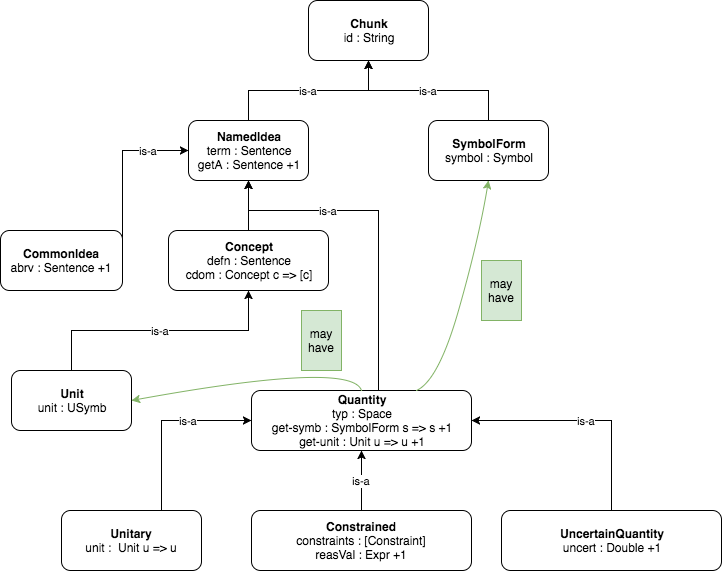
\includegraphics[width=0.5\textwidth]{figures/class_hierarchy.png}
    \caption{Drasil chunk hierarchy}
    \label{hierarchy}
\end{figure}

We can think of chunks as our building blocks of knowledge; they are the 
ingredients to be used in our \textit{Recipes}. Our language of recipes is a 
Domain-Specific Language (DSL) embedded in Haskell that is used to define what 
we would like to generate, and in what order. A small snippet of recipe 
language code for our Software Requirements Specification (SRS) can be seen in 
Figure~\ref{recipeLang}. This code is used to generate the \textit{Reference 
Materials} section of our SRS, which contains an introduction followed by the 
table of units, table of symbols, and table of abbreviations and acronyms 
subsections.

\begin{figure}
\begin{lstlisting}[language=Haskell, frame=single, showstringspaces=false, basicstyle=\small]
mkSRS :: DocDesc 
mkSRS = [RefSec (RefProg intro 
    [TUnits, 
    tsymb [TSPurpose, SymbOrder], 
    TAandA])]
        ...
\end{lstlisting}
\caption{The reference material section for an SRS written in Drasil's Document 
Language}
\label{recipeLang}
\end{figure}

The document generation language is fairly abstract (it knows about sections,
and subsections, various kinds of tables, and a variety of material typical
of SRSes), and allows for a
high degree of customization. Drasil also contains a code-generation language
integrating GOOL~\cite{Costabile2012} -- a Generic Object-Oriented Language -- which can
generate code in a number of different target languages including Python, Lua,
and C++.  We will discuss code generation in more depth through the example in
Section~\ref{SecGlassBR}.

Finally, there is the knowledge-base for Drasil (located in a series of
modules in the \lstinline|Data.Drasil| namespace). We 
are creating a database of reusable scientific knowledge that can be applied 
across a number of different applications across multiple domains. As the 
Drasil framework grows, we hope to continue to expand this database into an 
ontology of scientific knowledge for a number of disciplines. See 
Figure~\ref{ontology} for an example of some of the domains in which we have 
started to capture knowledge.

\begin{figure}
    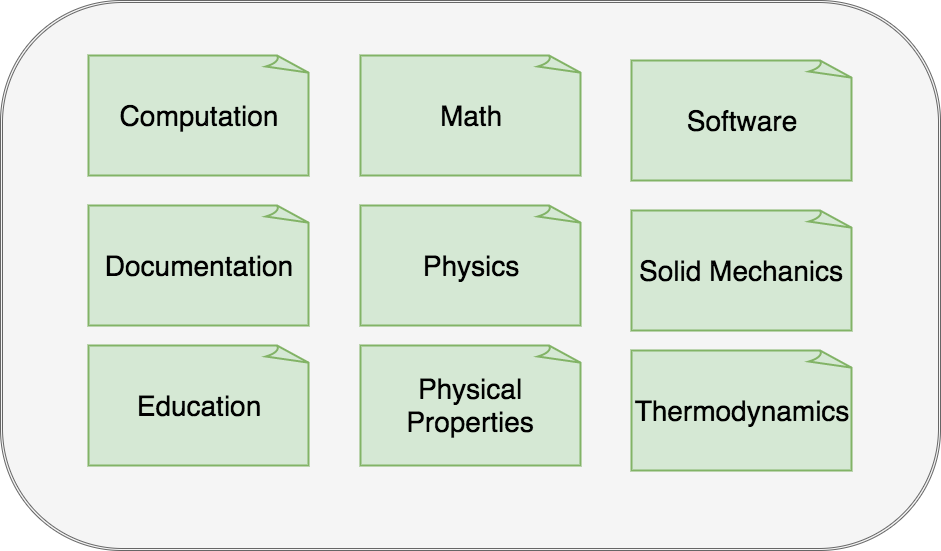
\includegraphics[width=.5\textwidth]{figures/ontology.png}
    \caption{Data.Drasil knowledge domains}
    \label{ontology}
\end{figure}

\section{Development Process for Drasil} \label{SecDevProcess}

We use an example-driven process -- where the examples are all reimplementations
of third-party software.  This grounds our efforts, and ensures that we are
able to reproduce real work rather than just toy examples.
We currently use five different examples, which are being worked on concurrently,
to drive the development of Drasil:

\begin{itemize}
\item Chipmunk2D Game Physics Engine
\item Solar Water Heating System Incorporating Phase Change Material (PCM)
\item Solar Water Heating System (No PCM)
\item Slope Stability Analysis (SSP)
\item Glass Breakage Analysis (GlassBR)
\end{itemize}
The original (non-Drasil) documentation for these examples came out of a study
on Document Driven Design (DDD) for SCS~\cite{SmithJegatheesanAndKelly2016}.

Our approach allows us the flexibility to prototype without 
over-designing. As a new feature becomes necessary to continue the 
implementation of a given example, only then do we design, test, implement, and 
re-test it. We occasionally implement features we may need in the future, but 
only in those instances when it is obvious that we are taking the right 
approach.  Five examples are enough to see ``patterns'' emerging
in different examples, which drive further design.

The five examples have also shown themselves to be an ideal means to bring
additional members on to the project.  Summer student research assistants
joined the project and were responsible for completing most of the work on
translating the original examples into Drasil, and then later transforming the
examples, as the Drasil DSLs have been extended and refactored.  Through their
work, the students have demonstrated that using Drasil does not require prior
knowledge of Haskell and code generation techniques.  These students come from
a variety of disciplines -- Chemical Engineering, Applied Mathematics, Computer
Science and Software Engineering, with levels of education ranging from first
to third year of an undergraduate program. None of the students had prior 
knowledge of Haskell. Yet all picked up the ideas quickly, and were able to make 
very significant contributions. Most were already able to make contributions on 
their second day of work -- and some were able to do substantial changes to the 
infrastructure too.

The current incarnation of the Drasil framework can be found on GitHub at 
\href{https://github.com/JacquesCarette/literate-scientific-software}
{https://github.com/JacquesCarette/literate-scientific-software}. We use code
peer-reviews throughout the development to correct missteps early on, and 
keep an up-to-date issue tracker for any bugs, feature requests, or other 
``to-do'' tasks. This has been an invaluable means of communication, 
especially when various team members were travelling, or simply working
asynchronously.

There are two means for prodding the development of Drasil:  first, the
usual ``wouldn't it be nice if we had feature X''.  Second, and more
importantly, a frequent \emph{introspection} of the code, encoding of the
examples, recipes, etc, to find patterns of use.  This has led to many
refactorings.  But it has also led us to \emph{de-embed} knowledge from
recipes and examples into re-usable chunks.  And of course, once patterns
are found and abstracted, often this reveals new patterns.

By adopting a practical, example-driven, ``bottom-up,'' approach for the
development of Drasil, we have avoided some of the problems inherent in a more
theoretical, or ``top-down,'' approach.  The size, scope and complexity of SCS
means that attempting to imagine a priori the DSLs we would need would be
exceedingly difficult.  We would invariably leave something out and likely
provide too simple a framework -- or spend a huge amount of time designing
features that turn out not to be needed in practice.  Rather than try to
arbitrarily determine the initial scope of Drasil, we let the examples tell us
what they need. The ``bottom-up'' approach was previously successfully used for
generating members of the family of Gaussian elimination
algorithms~\cite{Carette2006}, as well as a generator for geometry
kernels~\cite{CaretteEtAl2011}.

The idea that scientific software forms a program
family~\cite{SmithMcCutchanAndCao2007} is helpful for the current work.  We can
imagine that each of our five examples provides one specific instance of the
more general family of SCS.  With five examples we feel confident that enough of
the commonalities and variabilities between members of the family of SCS are
present that the initial implementation of Drasil will provide a reasonable
starting point for implementing a representative subset of the full family of
SCS.

\section{A Practical Example (GlassBR)} \label{SecGlassBR}

GlassBR is software used by structural engineers to predict whether or 
not a slab of glass will be able to withstand a given explosion without
breaking.  

This software is fairly simple; it has two (structured) inputs, the 
glass geometry and blast type, and a tolerance (the allowed probability
of breakage). The first two are comprised of
a number of fields (glass type, dimensions, TNT equivalent factor, 
standoff distance, etc.).

The output of GlassBR is whether or not the glass slab is considered safe,
determined by calculating the probability of breakage.  This calculation involves
interpolation from several tabulated values, as some of the quantities have
as yet not well-accepted models beyond empirical interpolation from experiments.

We will follow one specific piece of knowledge through from requirements to
code, as a means to illustrate the use of Drasil.

\begin{figure}
\begin{center}
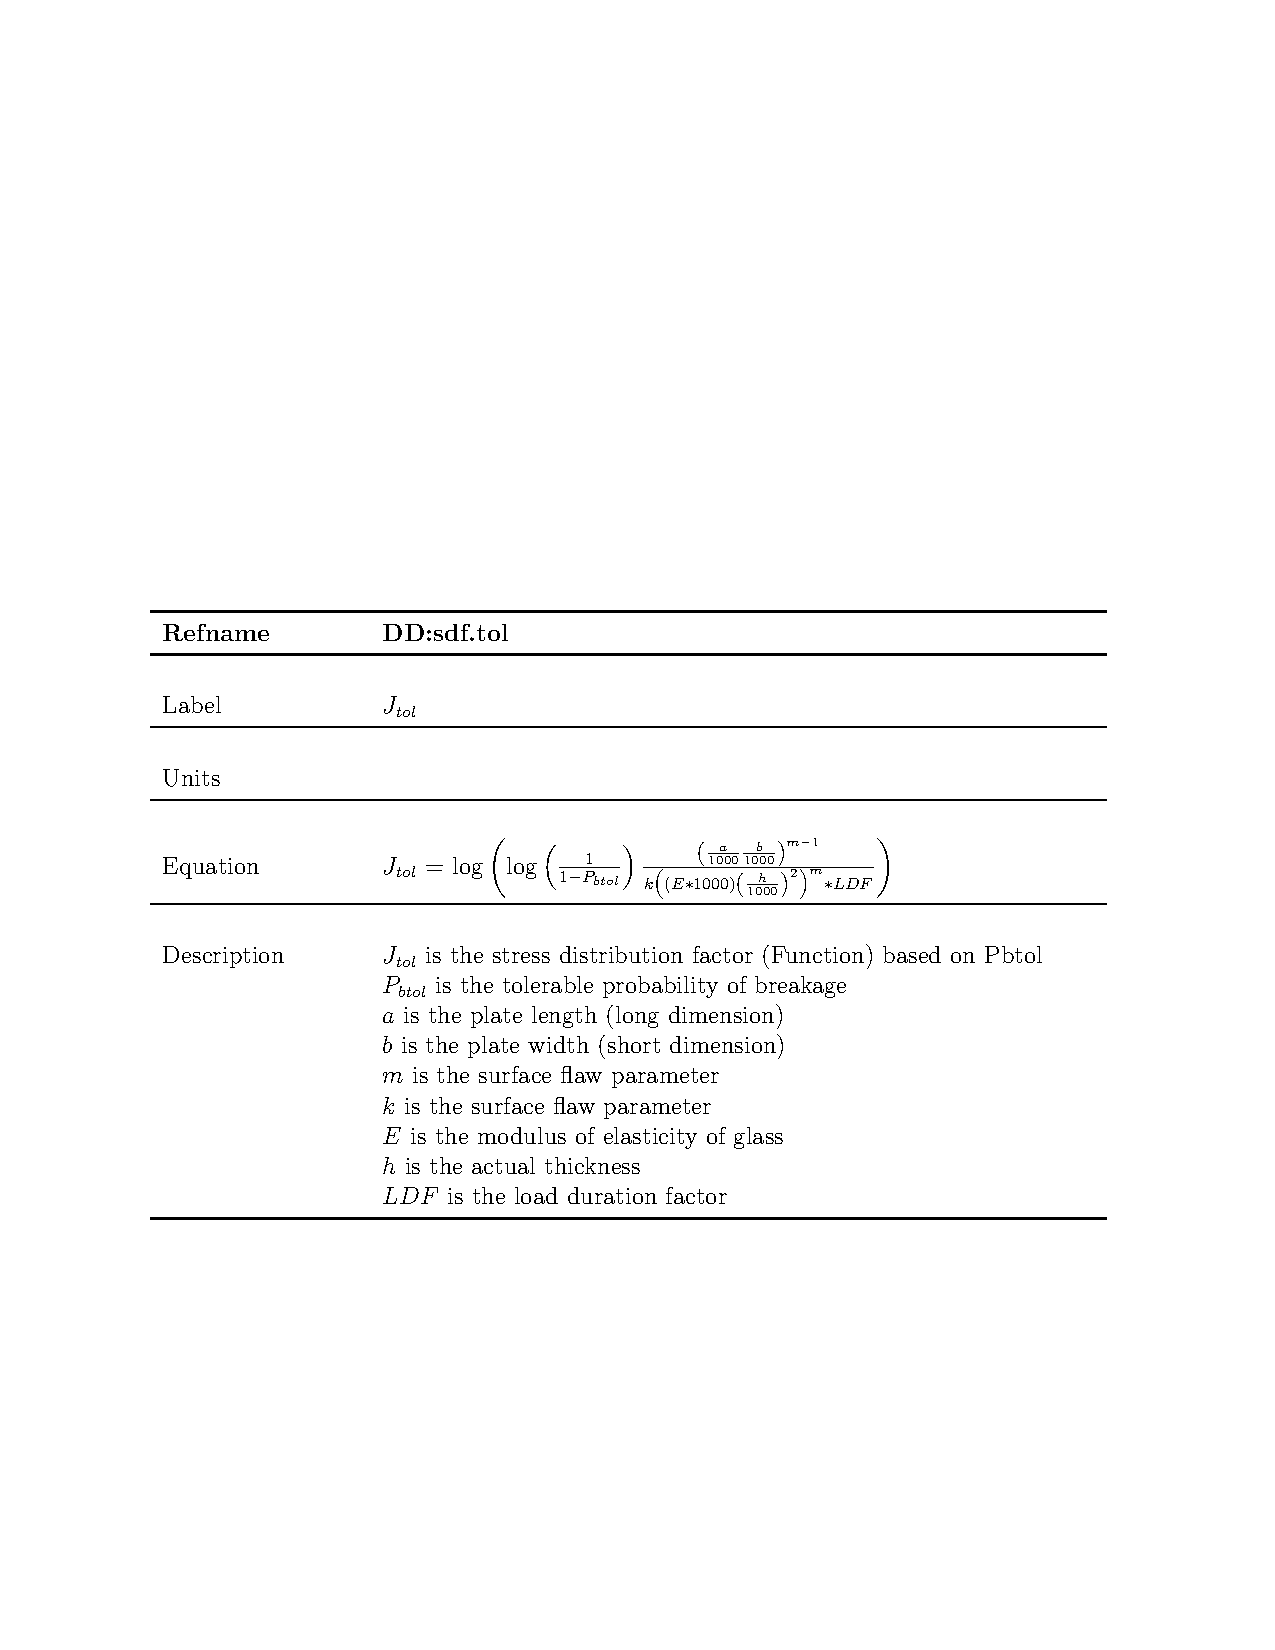
\includegraphics[width=0.45\textwidth]{./figures/Jtol_pdf.pdf}
\end{center}
\caption{\jtol{} from GlassBR Requirements}
\label{Fig_Jtolpdf}
\end{figure}

Let us start by taking a look at a data definition for the tolerable stress
distribution factor (\jtol{}) for GlassBR. Figure~\ref{Fig_Jtolpdf} shows
\jtol{} as rendered by \texttt{pdflatex}, from the Drasil-generated \LaTeX 
that came from the \jtol{} quantity chunk. We can also generate the documents
in HTML. The data definition is part of the requirements for the GlassBR
software.  As this requirement is in the form of a (solved) equation, it is
straightforward to generate code to
calculate \jtol{} from this.  A python version of this code can be seen in
Figure~\ref{Fig_JtolPython}). From the \jtol{} quantity chunk, we can generate
this code as well as the documentation!  Not only that, but thanks to the
incorporation of GOOL, we can also generate Java, Lua, C\#, etc. We present
the generated C\# code for reference in Figure~\ref{Fig_JtolCS}.

 \begin{figure*}
 \begin{lstlisting}[language=python, frame=single, showstringspaces=false, basicstyle=\small]
def calc_j_tol(inparams):
  j_tol = math.log((math.log(1.0/(1.0 - inparams.pbtol))) * 
     ((((inparams.a / 1000.0) * (inparams.b / 1000.0)) ** (inparams.m - 1.0)) / 
     ((inparams.k * (((inparams.E * 1000.0) * 
     ((inparams.h / 1000.0) ** 2.0)) ** inparams.m)) * inparams.ldf))) 
  return j_tol
 \end{lstlisting}
 \caption{Python code to Calculate \jtol{}}
 \label{Fig_JtolPython}
 \end{figure*}
 
\ds{We have options for C\#, Java, C++, and Python gen'd code.}
\begin{figure*}
\begin{lstlisting}[frame=single, showstringspaces=false, basicstyle=\small]
public static double J_tol(InputParameters inParams, double h, double LDF) {
    return Math.Log((Math.Log(1 / (1 - inParams.P_btol))) * 
        ((Math.Pow(inParams.a / 1000 * inParams.b / 1000, Constants.m - 1)) / 
        (Constants.k * ((Math.Pow(Constants.E * 1000 * (Math.Pow(h, 2)), Constants.m)) * LDF))));
}
 \end{lstlisting}
 \caption{Generated C\# code to Calculate \jtol{}}
 \label{Fig_JtolCS}
 \end{figure*}
 


%\spr{In reference to Figure 5:  The code that was here was the output of the 
%manually written GOOL code.  I switched it to 
%what is currently being generated (I assume this is supposed to be the generated 
%code?  If not
%I left the original version commented out).}
%\ds{It was meant to be the incorrect (due to unit conversion using 1000*) code, 
%whether manually written or generated. We did not refer to it as ``generated" code.}
%\begin{figure*}
%\begin{lstlisting}[language=python, frame=single, showstringspaces=false]
%def J_tol(inParams, h, LDF):
%    return math.log((math.log(1 / (1 - inParams.P_btol))) * (((inParams.a * inParams.b) ** 
%    (Constants.m - 1)) / (Constants.k * (((Constants.E * (h ** 2)) ** Constants.m) * LDF))))
%\end{lstlisting}
%\caption{Python code to Calculate \jtol{}}
%\label{Fig_JtolPython}
%\end{figure*}

The source knowledge for generating both the documentation and the code has been
captured using chunks, as shown in Figure~\ref{Fig_JtolDrasil}. The value of
\jtol{} is calculated from the {\inlHask{tolStrDisFac_eq}} expression, which is
part of the {\inlHask{tolStrDisFac}} chunk.  The equation ({\inlHask{tolStrDisFac_eq}}) is
defined using other quantity chunks, like {\inlHask{plate_len}} and
{\inlHask{mod_elas}}.  These chunks themselves have their own definitions, which
includes their description, symbol and units.  When the knowledge from \jtol{} is
rendered in some form, the knowledge from its constituent chunks is also
available.  This means the \emph{Description} field in Figure~\ref{Fig_Jtolpdf} 
can be generated automatically from the knowledge implicit in the 
{\inlHask{tolStrDisFac_eq}} equation.

% \jc{lots of parens were removed. Some have been removed from the GlassBR source
% as well, they were not needed.}
\begin{figure*}
\begin{lstlisting}[language=Haskell, frame=single, showstringspaces=false, basicstyle=\small] 
stressDistFac = makeVC 
  "stressDistFac" (nounPhraseSP $ "stress distribution" ++ " factor (Function)") cJ

sdf_tol = makeVC 
  "sdf_tol" (nounPhraseSP $ "stress distribution factor (Function) based on Pbtol") 
  (sub (stressDistFac ^. symbol) (Atomic "tol"))

tolStrDisFac_eq :: Expr
tolStrDisFac_eq = log (log (1 / (1 - C pb_tol)) * ((Grouping ((C plate_len / 1000) * 
  (C plate_width) / 1000)) :^ (C sflawParamM - 1) / (C sflawParamK * 
  (Grouping (Grouping (C mod_elas * 1000) * 
  (square (Grouping (C act_thic) / 1000))))) :^ (C sflawParamM) * (C loadDF))))

tolStrDisFac :: QDefinition
tolStrDisFac = mkDataDef sdf_tol tolStrDisFac_eq
\end{lstlisting}
\caption{Drasil (Haskell) code for \jtol{} Knowledge}
\label{Fig_JtolDrasil}
\end{figure*}

To facilitate potential future change, Figure~\ref{Fig_JtolDrasil} shows that
the symbol for \jtol{} is defined as {\inlHask{sub (stressDistFac ^. symbol)
    (Atomic "tol")}.  This means the symbol for \jtol{} is the symbol for the
  {\inlHask{stressDistFac}} with the subscript {\inlHask{"tol"}}.  If the symbol
  for {\inlHask{stressDistFac}} should change from $J$ to some other letter, the
  change in the base symbol and its variations will automatically be consistent
  throughout all artifacts.

During the process of translation from the original
documentation~\cite{SmithJegatheesanAndKelly2016} to the Drasil code, we noticed
an error in the code and documentation. The formula for \jtol{} should not
include the unit conversion implied by dividing by 1000 in a number of
places. Luckily, with one quick change to {\inlHask{tolStrDisFac_eq}} (shown in
Figure~\ref{Fig_JtolDrasil_fix}), we have corrected the error in our
knowledge-base. After re-running the generator, our code and documentation has
now been fixed and remains consistent.  With Drasil, we are able to correct an
error in one place (in the knowledge-base) and every artifact that depends on
that knowledge is automatically fixed.

\begin{figure*}
\begin{lstlisting}[language=Haskell, frame=single, showstringspaces=false, basicstyle=\small]
tolStrDisFac_eq :: Expr
tolStrDisFac_eq = log (log (1 / (1 - C pb_tol)) * ((Grouping (C plate_len * 
  C plate_width)) :^ (C sflawParamM - 1) / (C sflawParamK * 
  (Grouping (C mod_elas * square (C act_thick))) :^ (C sflawParamM) * (C loadDF))))
\end{lstlisting}
\caption{Modified Drasil (Haskell) code for \jtol{} equation}
\label{Fig_JtolDrasil_fix}
\end{figure*}

Similarly to the knowledge for \jtol{}, we have captured all of the knowledge
pertaining to GlassBR in chunks. Many of the chunks pertaining to documentation
concepts were previously captured in our knowledge-base, under
Data.Drasil.Concepts.Documentation, and are being reused in the GlassBR
implementation. Figure~\ref{Fig_docConcepts} shows a number of these chunks. The
chunks shown are all \textit{NamedChunks}, an instance of the \textit{NamedIdea}
class, which have been constructed using other, smaller chunks of knowledge. In
the case of \inlHask{prpsOfDoc}, we have used a special combinator,
`\inlHask{of_}', for increased readability.

\begin{figure}%[p]
\begin{lstlisting}[frame=single, showstringspaces=false, basicstyle=\small, upquote=false]
physicalConstraint = compoundNC physical constraint
physicalProperty   = compoundNC physical property
physicalSystem     = compoundNC physical system
problemDescription = compoundNC problem description
productUC          = compoundNC product_ useCase
safetyReq          = compoundNC safety requirement_
softwareConstraint = compoundNC software constraint
...
prpsOfDoc = npnc "prpsOfDoc" 
    (purpose `of_` document)

\end{lstlisting}
\caption{An excerpt of Documentation Concept chunks}
\label{Fig_docConcepts}
\end{figure}

The knowledge used by GlassBR can be assembled and extracted in different ways
to produce a multitude of views, i.e. our artifacts, including the SRS. For a
sense of what we can generate from this knowledge, see the table of contents for
the currently generated GlassBR SRS (Figure~\ref{Fig_ToCGlassBRSRS}). The SRS
template for GlassBR, and the other four examples, follows that from Smith and
Lai~\cite{SmithAndLai2005}, although a different recipe could be used to
generate an alternate view of the requirements.  For instance, the requirements
documentation generated for some audiences could provide less detail on equation
derivations.  Again, our documents can be generated in TeX and/or HTML for more
flexibility. Both contain automated internal referencing.

\begin{figure}
\begin{center}
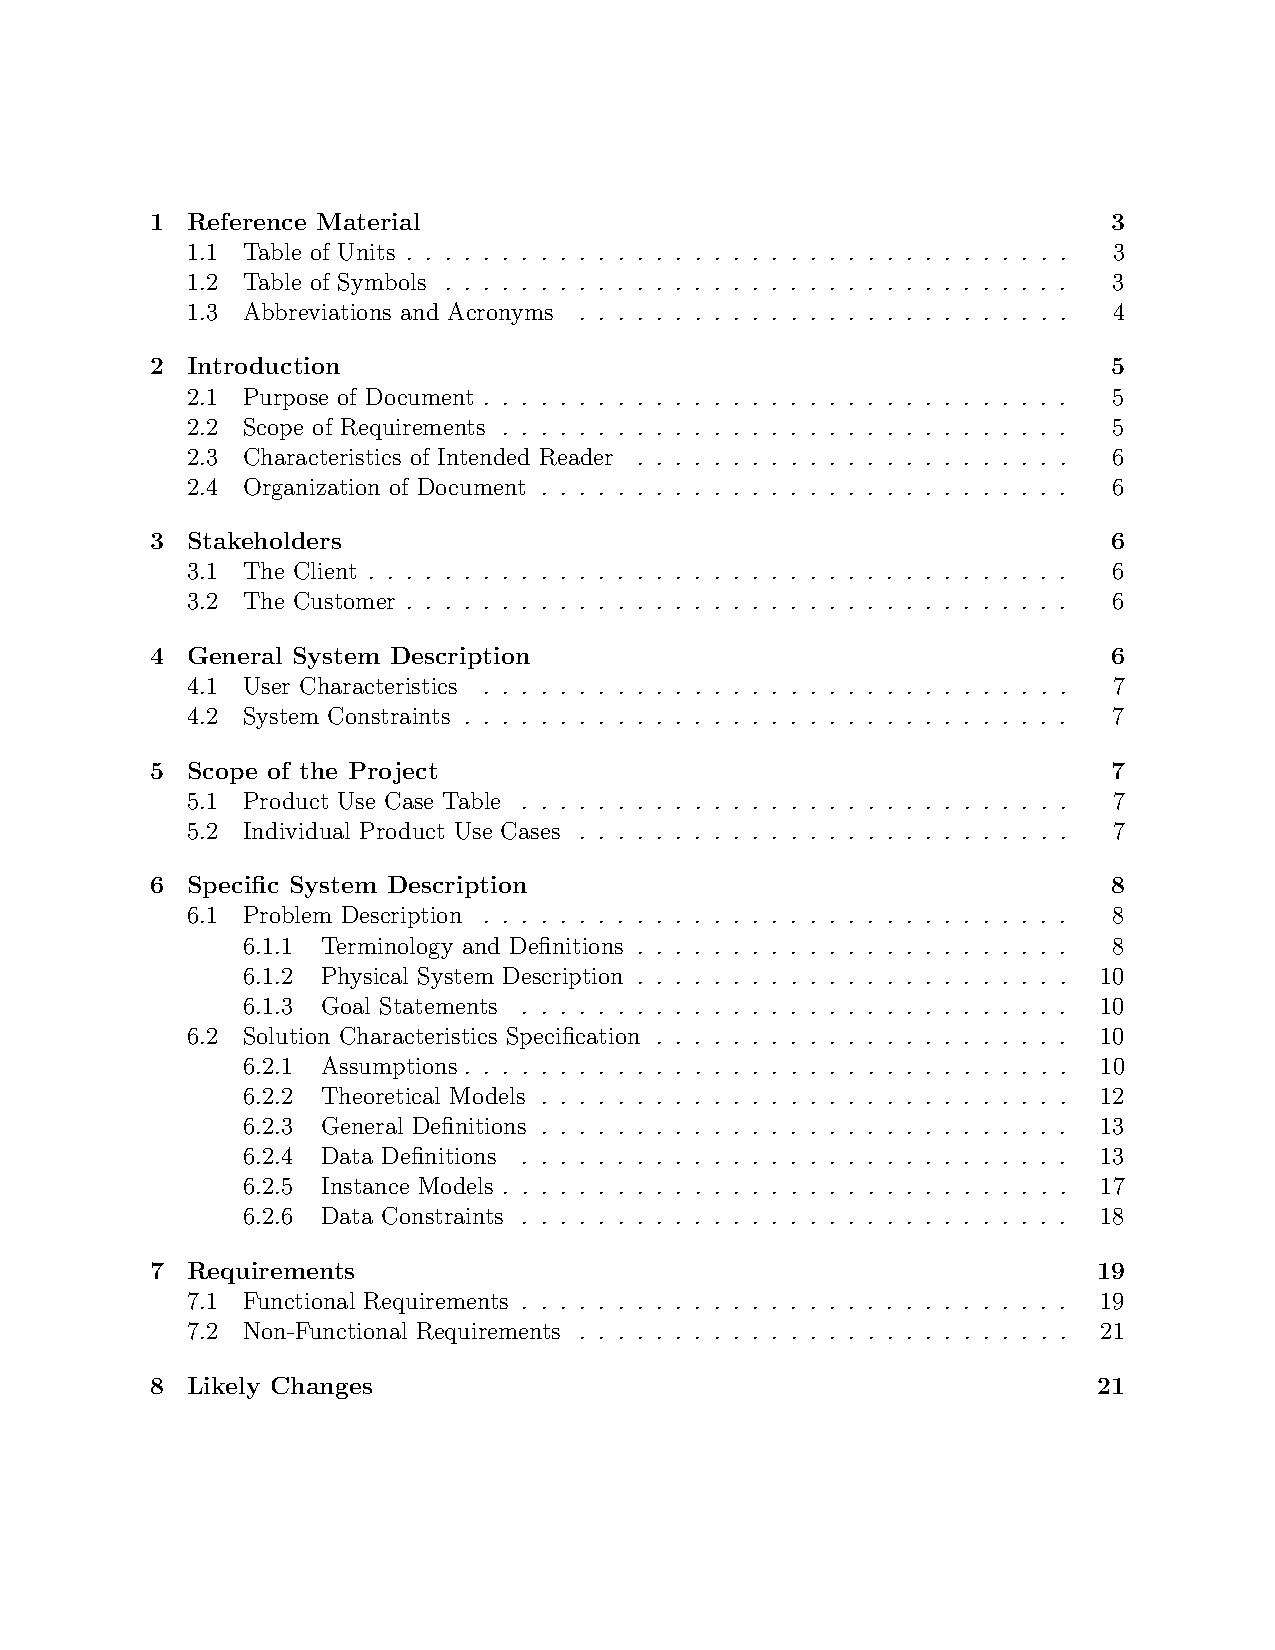
\includegraphics[scale=0.5]{./figures/TofC.pdf}
\end{center}
\caption{Table of Contents for Generated SRS for GlassBR}
\label{Fig_ToCGlassBRSRS}
\end{figure}

Another thing to note in our SRS is that the traceability information between
definitions, assumptions, theories, and instance models is automatically 
generated, including the traceability graph shown in 
Figure~\ref{Fig_TraceGraph}.

\begin{figure}
\begin{center}
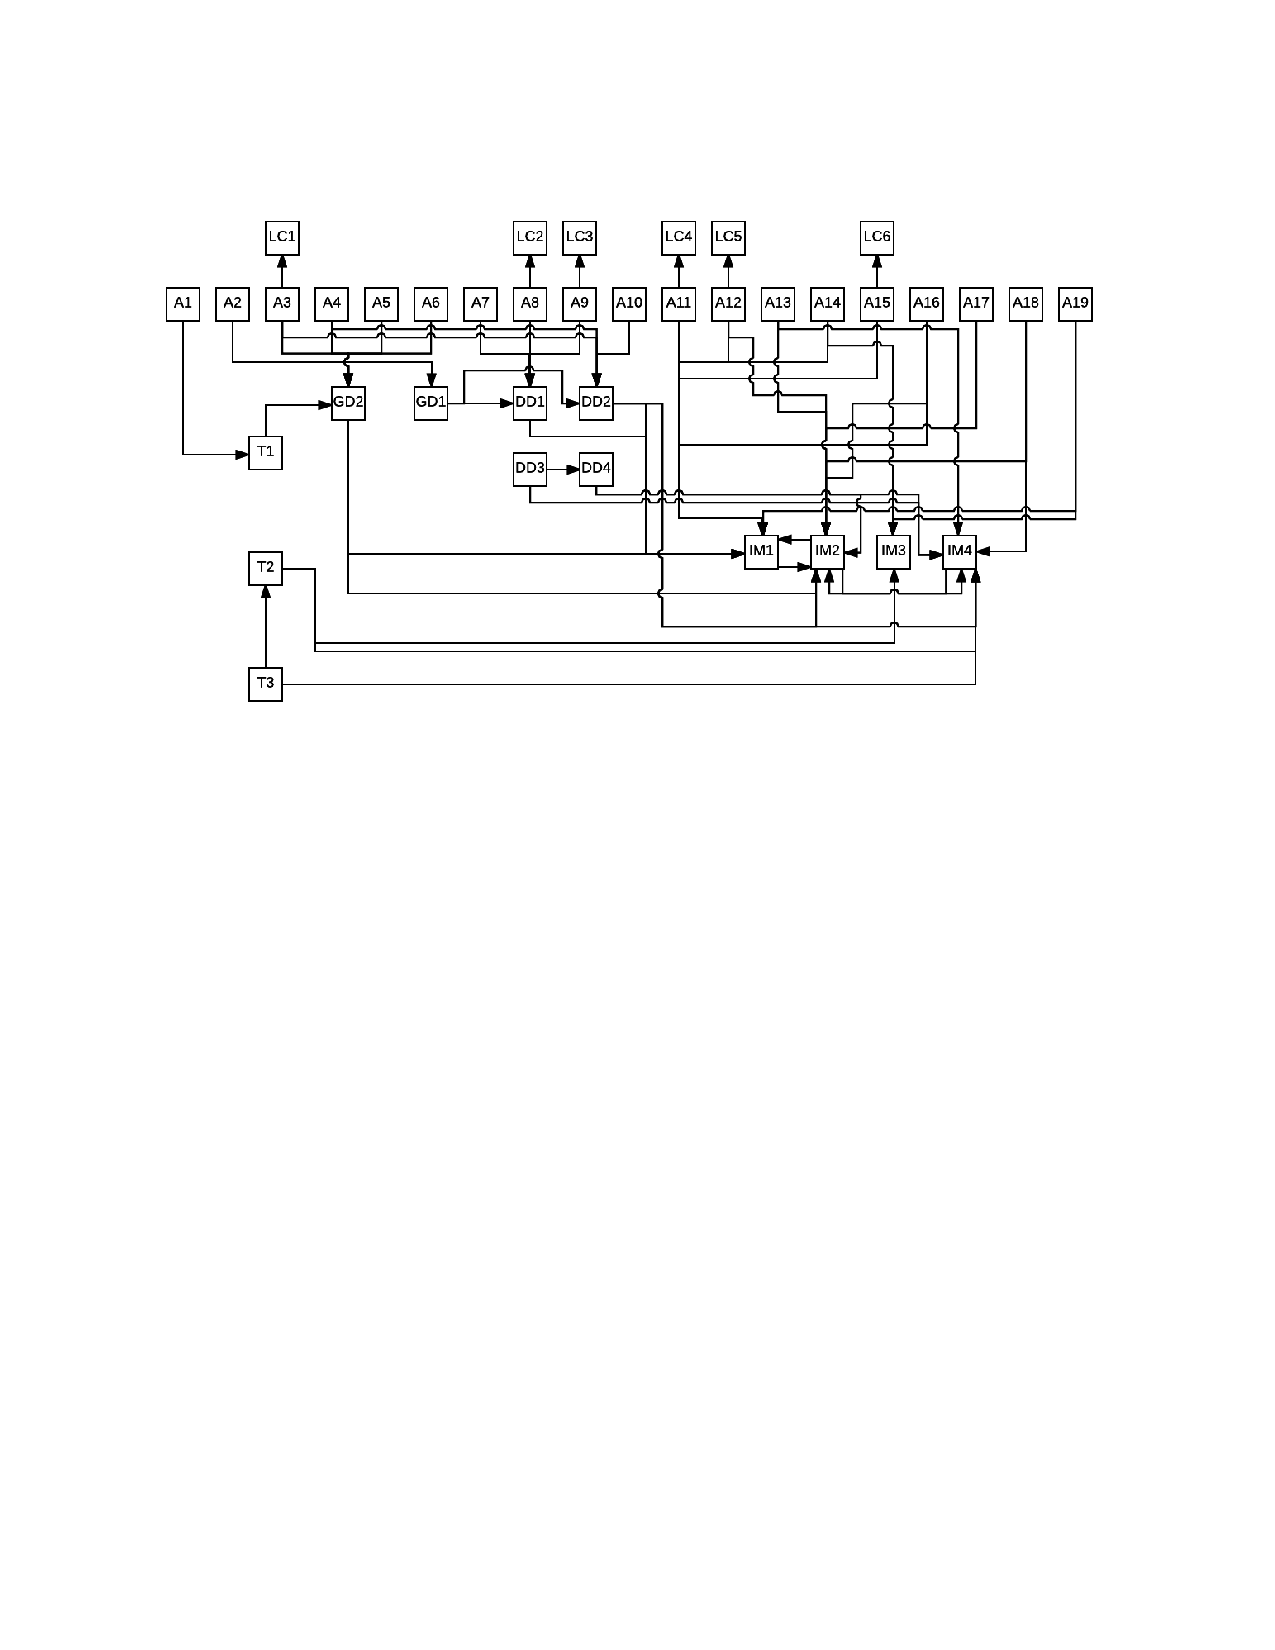
\includegraphics[scale=0.5]{./figures/TraceGraph.pdf}
\end{center}
\caption{Traceability Graph}
\label{Fig_TraceGraph}
\end{figure}

\section{Quality Improvements} \label{SecQuality}

Throughout Drasil's development lifecycle, we have already noticed a number of 
non-trivial quality improvements to the software examples being re-developed. 
These improvements come in a wide range of areas, but for the sake of brevity 
we will focus on certifiability, reusability, and reproducibility.

\subsection{Certifiability}

Certifying (or re-certifying) software can be a lengthy and expensive process
where a single error can cause the software to fail the certification process.
Consider the following equation from our solar water heating example which
states that energy in the water must be conserved between the heating coil and
water, and water and PCM (Phase Change Material):

\begin{equation*}
E_W = \int_{0}^{t} h_C A_C (T_C - T_W(t)) dt - \int_{0}^{t} h_P A_P (T_W(t) - T_P(t)) dt
\end{equation*}
%\wss{We need to define the terms in this equation.}  
\noindent where:
\begin{itemize}
    \item $E_W$ is the change in heat energy in the water
    \item $A_C$ is the heating coil surface area
    \item $A_P$ is the PCM surface area
    \item $h_C$ is the convective heat transfer coefficient between coil and 
    water
    \item $h_P$ is the convective heat transfer coefficient between PCM and 
    water 
    \item $T_C$ is the temperature of the heating coil
    \item $T_P$ is the temperature of the PCM
    \item $T_W$ is the temperature of the water
\end{itemize}

This is trivial for a human to check, and writing code to automatically check it
during the software execution is also very simple. However, it is still
time-consuming and should it ever need to change, such as if there is a change
in the assumption that the tank is a perfect insulator, it would require
developers to make a number of modifications to many artifacts in the future.

\begin{table} 
\centering
\caption{Constraints on Quantities -- Used To Verify Inputs}
\begin{tabular}{c c r c } 
\toprule
\textbf{Var} & \textbf{Constraints} & \textbf{Typical Value} & \textbf{Uncertainty}\\ \midrule
$L$ & $L > 0$ & 1.5 m & 10\% \\ 
$\rho_P$ & $\rho_P > 0$    & 1007 kg/m$^3$    & 10\% \\
\bottomrule
\end{tabular}
\label{tab:pcm}
\end{table}

Thanks to Drasil's knowledge-capture mechanisms, we can capture the above 
equation in one place, thus any changes can be made very quickly. Not only 
that, but sanity checks (such as ensuring constraints on inputs) can also be 
captured and reused. An example of these sorts of sanity checks can be seen in 
Table~\ref{tab:pcm}. They include hard physical constraints, ex. $L > 0$, as 
well as typical values. Capturing this information
delivers a wider array of advantages, including:

\begin{itemize}
\item Generating guards against invalid input automatically
\item Generating certain test cases automatically
\item Generating views suitable for inspection
\item Warning the user if they choose a value that is order(s) of magnitude
  different than the typical value
\end{itemize}
We can also see that it is straightforward to trace changes and verify that they 
are correct, thanks to our one-source, generative approach. We can produce 
documents similar to those commonly found in literate programming where we 
display the equations and code implementations (example: the \jtol{} equation 
and the python code used to calculate it) side-by-side, allowing a human to 
quickly verify the code is correct.  This literate technique proved valuable with
the nuclear safety analysis software mentioned
earlier~\cite{SmithAndKoothoor2016}.

We have also touched on one of the greatest advantages (implied 
earlier): 
\fbox{If there is an error somewhere, it is wrong everywhere.}

This 
may seem like a disadvantage, but ensuring every artifact contains the same 
errors means there is a much greater chance of those errors being spotted. In 
our experience, many examples of software include code that does not match the 
design (due to hacks, last-minute changes, etc.), and an error that would 
hamper certification efforts can fly under the radar. 

For (re-)certification purposes, we want to be able to find any and all errors, 
trace them to their source, and fix them quickly. Drasil has shown great 
promise in that respect.

\subsection{Reusability}

Reusability is a core tenet of Drasil's development. This can be seen most
obviously in the knowledge-capture mechanisms we have created. These mechanisms
facilitate reuse through common knowledge databases for each domain (recall
Figure~\ref{ontology}).  The reuse can occur within a single document, with a
series of documents, and even between projects.

The value of reuse within a given document is seen in Figure~\ref{Fig_Jtolpdf}
and Figure~\ref{Fig_ToCGlassBRSRS}.  Information on variables, including their
definitions, their symbols and their units, is reused in multiple locations
throughout the requirements document (SRS).  For instance, lists of variables
appear in the table of symbols, as part of each data definition and as part of
the instance models.  Maintaining the consistency between these different
renderings would be very challenging manually, but by reusing the knowledge
whenever necessary, the documentation is significantly more maintainable.

Consider the following software artifacts typically found in a rational design 
process for software development~\cite{ParnasAndClements1986}:

\begin{itemize}
\item Software Requirements Specification (SRS)
\item Module Interface Guide (MIS)
\item Source Code
\item Test cases
\end{itemize}

Within these artifacts, there is considerable duplication of specific knowledge 
related to the software being designed. Knowledge from the SRS will appear, 
possibly transformed, throughout each of the other artifacts. We seek to 
de-embed specific knowledge from within any one artifact to easily reuse 
it throughout them all. This knowledge includes, but is not limited to:

\begin{itemize}
\item Scientific Knowledge
\item Models
\item Units
\item Symbols
\item Descriptions
\item Traceability information
\end{itemize}

While implementing our case studies in Drasil, we have found this de-embedding 
process to be invaluable. Previously ``dead'' information found in the software 
artifacts is now captured, reusable, and transformable. For example, an equation 
such as the one for defining \jtol{} can now be reused across artifacts in 
whatever form we deem necessary. This could be the equation written 
mathematically, described in English, or converted into executable code. Every 
form is still being generated from the same source, we simply reuse it in a 
slightly different way.

Reusing knowledge across artifacts in one software project is already 
incredibly useful, however, we have taken it a step further. Drasil allows us 
to reuse between projects. We can reuse a family of related models, or reuse 
pieces of knowledge from a given domain as necessary. Consider the vast number 
of software projects that rely on interpolation, or must ensure conservation of thermal 
energy. We can capture this knowledge once and reuse it through all of these 
projects.

We have already begun using knowledge across projects with great results. Our
two implementations of the solar water heating systems (one with PCM and one
without) have a vast amount of overlap in the requisite knowledge.  The same
governing equations, such as conservation of thermal energy, apply, but in a
simplified form when one does not have to worry about heat transfer to and phase
change of, the PCM. As such, these two implementation utilize many of the same
chunks from our knowledge-base, simply reordered and transformed as
necessary. If we find an error in the theory, or need to make a change to
improve the validity of our calculations, fixing the Drasil source will update
both projects (and any other members of the program family) simultaneously.  

\subsection{Reproducibility}

Typically when we refer to reproducibility, the emphasis is on reproducing the
calculations from compiled code. The problem is that over time programming
languages, compilers and operating environments change.  Virtual Machines (VMs)
can be a significant help here, but VMs do not help when there are problems in
the original code.  What if our trust in the original code is in doubt?  What if
we need to reproduce the results not starting from the code, but starting from
the original theory?  Unfortunately, multiple examples
exist~\cite{CrickAndHall2014, IonescuAndJansson2013} where results from research
software could not be independently reproduced, due to a need for local
knowledge missing from published documents.  Examples of missing knowledge
includes missing assumptions, derivations, and undocumented modifications
to the code.  Should it not be easier to independently replicate the work of
others, without relying on the code they have written?

We want to replicate not only the execution of the code, but the whole of the 
software from theory to implementation. Given the appropriate theoretical 
knowledge, assumptions, equations, etc. we should be able to take this 
high-level knowledge and reproduce an implementation which will return 
consistent results. Drasil allows us to do exactly this; we can capture the 
high-level science knowledge and use it to reproduce a piece of software. We 
can also package our projects in a Drasil-ready format, such that the software 
can be generated on-the-fly by any who wish to replicate the results or 
double-check the science.

Drasil can also potentially check for completeness and consistency, ensuring 
the little things that are tedious, if trivial, to manually verify. For 
example: every symbol should be defined and used and should not change 
throughout the artifacts (inter- and itra-artifact consistency). This may seem 
minor, but one of our case studies, which had been reviewed by humans on 
numerous occasions, introduced a new symbol for an existing concept in a 
derivation. This new symbol was never defined and did not appear in the table of 
symbols. When implementing the project in Drasil, however, this error was made 
obvious almost immediately and was easily fixed.

Previously, the manual checks for verifying documentation have been
listed~\cite{SmithAndKoothoor2016}:
\begin{itemize}
\item check that every symbol is defined
\item check that every symbol is used at least once
\item check that every equation either has a derivation, or a citation to its
  source
\item check that every general definition, data definition, and assumption is
  used by at least one other component of the document
\item check that every line of code either traces back to a description of the
  numerical algorithm, to a data definition, to an instance model, to an
  assumption, or to a value from the auxiliary constants table in the SRS.
\end{itemize}
Going forward Drasil can be used to automate these checks and provide error or
warning messages when they are violated.

Overall, Drasil lends itself incredibly well to ensuring reproducibility in a 
much larger sense than we normally consider. It allows us to focus on the 
science, (re-)building our projects from the fundamental knowledge instead of 
relying on a lone developer's code. Drasil also forces all assumptions to be 
documented, and disallows local hacks, since the generated code should never be 
modified by a human, it should only be (re-)generated.

\section{Future Work} \label{SecFuture}

Drasil has come a long way in the last year, yet there is still much to be 
done. With the current code-generation mechanisms being fairly naive, we have 
begun work on a language of design which allows us to apply design decisions to 
the theory knowledge to produce more flexible code. This language allows us to 
classify design and implementation choices in a reusable manner and will 
allow us to progress with the generation of design documents, which are 
currently difficult to produce in Drasil.

The language of design will also facilitate more robust automated test case 
generation. By utilizing the captured design decisions, we will have a deeper 
knowledge of specific choices being made in our generated code. For example, in 
GlassBR, we will know which interpolation algorithm to use, and we will be able 
to generate test cases relevant to said algorithm.

%\spr{If you want to add more to this section, you could mention automated 
%verification.  Unit test generation isn't far away after generation is reliably working.  
%Also, we can start adding options to insert checks and guards into the generated
%code -- this ties into the design language.}

Another large feature that will be a necessity in the long-run, but has thus 
far been relegated to the back-burner, is a much more user-friendly syntax, or 
even a tool to aid in the creation of Drasil projects. Drasil is currently
fairly esoteric to use, even with all our documentation to date. Yet, with 
each iteration of the language we introduce new, simplifying abstractions, 
which have already made it easier to use. Our experience with our summer student 
research assistants is a testament to that. We are aware, however, of the gap 
that still needs to be closed before it will be ready for our target 
demographic.

We are also continuing work on:
\begin{itemize}
    \item Generating new types of software artifacts
    \item Implementing much larger examples
\end{itemize}

Thanks to our practical approach to Drasil's design, there will likely be many 
other minor features to add and changes to make that are not yet entirely clear 
to us.

\section{Concluding Remarks}

While Drasil is still a work-in-progress, it shows great promise as a tool to 
aid SCS developers. The ability to capture scientific knowledge, document it, 
and transform it into usable code from a single, fully-traceable source should 
not be underestimated.

We have already seen non-trivial improvements to existing software during its 
re-implementation in our current, working-copy of Drasil. The case studies are 
now easier to verify, maintain, reuse, and replicate than they were before. 
There is also far less ambiguity on where certain concepts originated, as 
everything is captured in one source (the knowledge-base).

Not only do we believe that scientists will be able to create higher quality
software while focusing more on the science; they will be able to replicate and
reuse each other's work in a far more robust manner than we currently see in
practice. We hope Drasil will solve the current problems with software result
replicability starting from the theory~\cite{CrickAndHall2014,
  IonescuAndJansson2013}.

Software (re-)certification will also become a far less daunting task in a
future with Drasil. With full traceability of information and the ability to 
generate new document views on-the-fly, we will be able to streamline the 
process.  This means that recertification will be significantly less expensive
than the original certification exercise.

While developing in Drasil does come with a fairly high, up-front investment of 
effort, we believe the long-term maintainability improvements, along with the 
streamlining of verification/certification and the other previously mentioned 
advantages are well worth the cost.

%\jc{Isn't Wael a first name?  Also, I think we should acknowledge all of
%the summer students by name.}

\begin{acks}

Drasil would not have progressed this quickly without the efforts of our
summer research assistants: Henry Madej, Aaron Mori, Maryyam Niazi,
Nicholas Richardson, and Daniel Scime.

The assistance of McMaster University's Dr.\ Manuel Campidelli, Dr.\ Wael 
El-Dakhakhni, and Dr.\ Michael Tait with the GlassBR example is
greatly appreciated.


\end{acks}

\bibliographystyle{ACM-Reference-Format}
\bibliography{SzymczakEtAl2017} 

\end{document}
